\documentclass[pdf]{beamer}
\usepackage[latin1]{inputenc}
\usepackage{multirow}
\usetheme{Warsaw} %Warsaw
\usecolortheme{beetle}

\begin{document}

\title[Post Analysis]{DNA Microarrays\\Post Analysis\\}
\subtitle{BCB 504: Applied Bioinformatics\\}
\author[Matt Settles]{Matt Settles}
\institute{University of Idaho\\ Bioinformatics and Computational Biology Program}
\date{\today}


%% Title page
\begin{frame}[plain]
  \titlepage
\end{frame}


%% Outline
\begin{frame}[plain] 
  \frametitle{Outline}
  \tableofcontents
\end{frame}

\section{Gene Ontology/Pathway Analysis}
\subsection{Gene Ontology}
\begin{frame}[allowframebreaks]
  \frametitle{Gene Ontology}
The Gene Ontology project is a major bioinformatics initiative with the aim of standardizing the representation of gene and gene product attributes across species and databases. T	he project provides a controlled vocabulary of terms for describing gene product characteristics and gene product annotation data from GO Consortium members, as well as tools to access and process this data. Read more about the \href{http://www.geneontology.org/}{Gene Ontology}.
\vspace{0.1in}

The Gene Ontology project provides an ontology of defined terms representing gene product properties. The ontology covers three domains: \textbf{cellular component}, the parts of a cell or its extracellular environment; \textbf{molecular function}, the elemental activities of a gene product at the molecular level, such as binding or catalysis; and \textbf{biological process}, operations or sets of molecular events with a defined beginning and end, pertinent to the functioning of integrated living units: cells, tissues, organs, and organisms.
\vspace{0.1in}

For example, the gene product cytochrome c can be described by the molecular function term oxidoreductase activity, the biological process terms oxidative phosphorylation and induction of cell death, and the cellular component terms mitochondrial matrix and mitochondrial inner membrane.
\vspace{0.1in}

Further, The GO ontology is structured as a directed acyclic graph, and each term has defined relationships to one or more other terms in the same domain, and sometimes to other domains. The GO vocabulary is designed to be species-neutral, and includes terms applicable to prokaryotes and eukaryotes, single and multicellular organisms.
\end{frame}

\subsection{Pathway}
\begin{frame}[allowframebreaks]
  \frametitle{Pathways}
Most common pathway resource is \textbf{\href{http://www.genome.jp/kegg/pathway.html}{KEGG}}, The Kyoto Encyclopedia of Genes and Genomes. However their FTP resource is no longer free as of Aug 2011, but their website and API is still free. 
\vspace{0.1in}

\textbf{\href{http://www.wikipathways.org/index.php/WikiPathways}{WikiPathways}} is another resource gaining some traction. Pathways are intended to represent interactions betweens genes (proteins).
\vspace{0.1in}

Most pathway resources have  significant amount of manual curation to them.

\end{frame}

\subsection{Analysis}
\begin{frame}[allowframebreaks]
  \frametitle{Microarray Analysis}
  Gene Ontology or Pathway Analysis is a data reduction technique used in order to summarize, or generalize results in a microarray experiment. It is not uncommone to either have hundreds, or even thousands, of differentially expresssed genes in an experiment. To summarize results on a gene by gene basis is not feasible and instead it is common to make more general statement based on Gene Ontologies or Pathways.
  \vspace{0.1in}
  
  The biological question being asked is typically:\\
  Are there Gene Ontologies (or Pathways) significantly over-represented (or under-represented) in my comparison as would be expected by chance. 

There are many R packages (Bioconductor) for both Pathway and Gene Ontology analysis, many of which work for both kinds of data.\\

Bioconductor Ontology based packages: \url{http://bioconductor.org/help/search/index.html?q=ontology}\\
Bioconductor Pathway based package: \url{http://bioconductor.org/help/search/index.html?q=pathway}\\

SigPathway package example:\\
\url{http://www.bioconductor.org/packages/2.12/bioc/vignettes/sigPathway/inst/doc/sigPathway-vignette.pdf}

\end{frame}


\section{Gene Co-Expression Network Analysis}

\begin{frame}[allowframebreaks]
	\frametitle{Weighted Gene Co-Expression Network Analysis (WGCNA)}

Many techniques employed for network based analysis (co-expression of genes), but my favorite is Dr. Horvath's (UCLA) approach.\\
\textbf{\url{http://labs.genetics.ucla.edu/horvath/CoexpressionNetwork/Rpackages/WGCNA/}}
\vspace{0.1in}

Briefly, computes the correlation matrix (expression) between all genes in a dataset, manipulates the correlation so that conform to a scale free discribution (\href{http://en.wikipedia.org/wiki/File:Scale-free_network_sample.png}{sfn}). Then Computes the topological overlap measure (TOM), ie connections are enhanced in a friend of a friend manner and translates this to a distance measure. Clusters (networks) of genes are determined by a dynamic cutting routine based on the heirarchical tree and k-means clustering results (hybrid-approach). These networks are then reduced by looking at their eigengenes (eigenvectors) and finnaly experimental parameters (phenotypes) can be associated with particular networks. In addition, genes within a network ranked by their connectivity, genes with high connectivity (central nodes) are assumed to be more important than other genes and may possibly represent gene targets.
\vspace{0.1in}

The WGCNA approach does however require a large number of samples, where the experimental conditions are expected to preturb gene expression. In other workds to develop networks you need to induce a pattern of gene expression across samples. 

\end{frame}

\section{Single Feature Polymorphisms}

\begin{frame}
\frametitle{Single Feature Polymorphisms (SFPs)}
When a short-oligonucleotide probe is designed at a position with a genomic or transcriptional polymorphism, the hybridization efficiency is reduced. SFPs are statistical differences in the probe level hybridization efficiency between two populations caused by an underlying genetic or transcriptional polymorphism. They are detected by comparing microarray probe level intensity signals, a proxy value for hybridization efficiency, between two populations. When hybridizing gDNA, SFPs are induced by single-nucleotide polymorphisms (SNPs) and small insertions/deletions (INDELS). When hybridizing mRNA, SFPs can also be induced by splicing variation and polyadenylation differences. 
\end{frame}

\begin{frame}[allowframebreaks]
\begin{center}
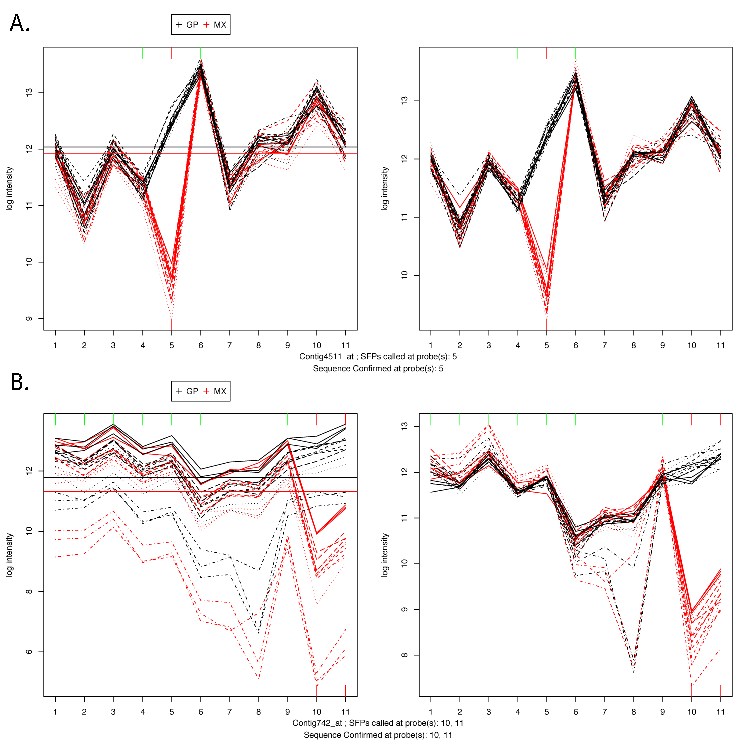
\includegraphics[scale=0.5]{figures/Figure1-SFP_plots.pdf} 
\end{center}
\end{frame}

\section{Single Feature Polymorphisms}
\begin{frame}[allowframebreaks]
\begin{center}
\includegraphics[scale=0.6]{figures/Figure6-SFPShiftedExp.pdf} 
\end{center}
\end{frame}

\section{Single Feature Polymorphisms}
\begin{frame}[allowframebreaks]
\begin{center}
\includegraphics[scale=0.6]{figures/Figure2-SFPpositionSensitivity.pdf} 
\end{center}
\end{frame}

\section{Single Feature Polymorphisms}
\begin{frame}[allowframebreaks]
\begin{center}
\includegraphics[scale=0.3]{figures/BB3geneXsfp.pdf} 
\end{center}
\end{frame}

% side by side frame
%\begin{frame}
%  \frametitle{The SAM table}
%  \begin{columns}[t] % contents are top vertically aligned
%    \begin{column}[T]{5cm} % each column can also be its own environment
%      \begin{itemize}
%        \item SAM table 
%        \item Can be created from the raw intensities, log intensities, model fitting residuals and other
%        \item Looking for large anomalies
%      \end{itemize}
%     \end{column}
%     \begin{column}[T]{5cm} % alternative top-align that's better for graphics
%       \includegraphics[scale=1.0]{figures/samtable.pdf} 
%     \end{column}
%  \end{columns}
%\end{frame}



%\frame{
%	\begin{description}
%	\item[Description]
%	A data driven approach for the computational and statistical understanding and expertise needed to solve bioinformatics problems that you will likely encounter in your research. 
%	\item[Goals]
%	Following this course the student will be capable of:
%	\begin{itemize} 
%		\item performing their own data analysis project, 
%		\item understanding the technical and statistical tools needed to conduct that analysis
%		\item have the computational ability to do the analysis
%		\item critically review and implement techniques and methods in publications.
%	\end{itemize}
%	\end{description}
%}
%
%\frame{

%\begin{frame}
%    \begin{columns}[c] % the "c" option specifies center vertical alignment
%    \column{.5\textwidth} % column designated by a command
%     Contents of the first column
%    \column{.5\textwidth}
%     Contents split \\ into two lines
%    \end{columns}
%\end{frame}
%
%\begin{frame}
%     \begin{columns}[t] % contents are top vertically aligned
%     \begin{column}[T]{5cm} % each column can also be its own environment
%     Contents of first column \\ split into two lines
%     \end{column}
%     \begin{column}[T]{5cm} % alternative top-align that's better for graphics
% Graphic would go here
%      \end{column}
%     \end{columns}
%\end{frame}
%
%\frame{
%   \begin{block}{This is a Block}
%      This is important information
%   \end{block}
% 
%   \begin{alertblock}{This is an Alert block}
%   This is an important alert
%   \end{alertblock}
% 
%   \begin{exampleblock}{This is an Example block}
%   This is an example 
%   \end{exampleblock}
%}

\end{document}
